\documentclass[11pt,oneside]{article}
\usepackage[a4paper,margin=25mm,headheight=15pt]{geometry}
\usepackage[T1]{fontenc}
\usepackage[utf8]{inputenc}
\IfFileExists{libertinus.sty}{\usepackage{libertinus}}{\usepackage{lmodern}}
\usepackage{microtype}
\usepackage{amsmath,amssymb,amsthm,mathtools,mathrsfs,bm}
\usepackage{booktabs,longtable,array,tabularx,multirow}
\usepackage{graphicx}
\usepackage{xcolor}
\usepackage{enumitem}
\usepackage{fancyhdr}
\usepackage{titlesec}
\usepackage{listings}
\usepackage{xurl}
\usepackage{hyperref}
\usepackage[nameinlink,noabbrev]{cleveref}
\usepackage{caption}

\definecolor{linkblue}{RGB}{25,75,135}
\definecolor{shadegray}{RGB}{246,247,249}
\definecolor{rulegray}{RGB}{195,201,208}
\definecolor{provedgreen}{RGB}{22,105,75}
\definecolor{conjectureorange}{RGB}{150,82,0}
\hypersetup{
  colorlinks=true,
  linkcolor=linkblue,
  citecolor=linkblue,
  urlcolor=linkblue,
  pdftitle={Dyadic-Comb Interpolation of the Fabius and Rvachev Functions},
  pdfsubject={Runge instability, endpoint-jet constraints, and stable local alternatives},
  pdfkeywords={Fabius function, Rvachev up-function, Lagrange interpolation, Hermite interpolation, Runge phenomenon, dyadic comb, Thue-Morse}
}

\pagestyle{fancy}
\fancyhf{}
\fancyhead[L]{\small Dyadic Fabius--Rvachev interpolation}
\fancyhead[R]{\small\nouppercase{\leftmark}}
\fancyfoot[C]{\thepage}
\renewcommand{\headrulewidth}{0.4pt}
\titleformat{\section}{\Large\bfseries}{\thesection}{0.7em}{}
\titleformat{\subsection}{\large\bfseries}{\thesubsection}{0.7em}{}
\titleformat{\subsubsection}{\normalsize\bfseries}{\thesubsubsection}{0.7em}{}
\setcounter{secnumdepth}{3}
\setcounter{tocdepth}{2}
\setlist[itemize]{leftmargin=2em,itemsep=0.25em,topsep=0.4em}
\setlist[enumerate]{leftmargin=2.3em,itemsep=0.25em,topsep=0.4em}
\setlength{\emergencystretch}{3em}

\newtheorem{theorem}{Theorem}[section]
\newtheorem{proposition}[theorem]{Proposition}
\newtheorem{lemma}[theorem]{Lemma}
\newtheorem{corollary}[theorem]{Corollary}
\newtheorem{conjecture}[theorem]{Conjecture}
\theoremstyle{definition}
\newtheorem{definition}[theorem]{Definition}
\newtheorem{algorithm}[theorem]{Algorithm}
\newtheorem{example}[theorem]{Example}
\newtheorem{question}[theorem]{Research question}
\theoremstyle{remark}
\newtheorem{remark}[theorem]{Remark}
\newtheorem{warning}[theorem]{Warning}

\newcommand{\R}{\mathbb R}
\newcommand{\C}{\mathbb C}
\newcommand{\Q}{\mathbb Q}
\newcommand{\N}{\mathbb N}
\newcommand{\Z}{\mathbb Z}
\newcommand{\Up}{\operatorname{up}}
\newcommand{\e}{\mathrm e}
\newcommand{\dd}{\,\mathrm d}
\newcommand{\wt}{\operatorname{wt}_2}
\newcommand{\bigO}{\mathcal O}
\newcommand{\smallo}{o}
\newcommand{\supp}{\operatorname{supp}}
\newcommand{\sgn}{\operatorname{sgn}}
\newcommand{\LambdaN}{\Lambda_{N,r}}
\newcommand{\EN}{E_N}
\newcommand{\eps}{\varepsilon}
\newcommand{\repo}{\texttt{Analysis/FabiusFunction/docs}}

\newenvironment{statusbox}[1]{%
  \par\smallskip\noindent\begin{center}\begin{minipage}{0.94\textwidth}%
  \hrule\vspace{0.5em}\noindent\textbf{#1}\par\smallskip
}{%
  \vspace{0.5em}\hrule\end{minipage}\end{center}\smallskip
}

\lstdefinestyle{pythonstyle}{
  language=Python,
  basicstyle=\ttfamily\footnotesize,
  backgroundcolor=\color{shadegray},
  frame=single,
  rulecolor=\color{rulegray},
  columns=fullflexible,
  keepspaces=true,
  showstringspaces=false,
  xleftmargin=0.7em,
  xrightmargin=0.7em,
  breaklines=true,
  aboveskip=0.8em,
  belowskip=0.8em
}

\title{\bfseries Dyadic-Comb Interpolation of the Fabius and Rvachev Functions\\[0.35em]
\large Runge instability, endpoint-jet constraints, exact arithmetic, and stable local alternatives}
\author{Research report for Vladimir Reshetnikov's \texttt{ProveIt} project}
\date{28 August 2026}

\begin{document}
\maketitle

\begin{abstract}
Let $N=2^n$ and interpolate the Fabius function $F$ at the additive dyadic comb
$x_j=j/N$, or Rvachev's compactly supported function $\Up$ at the affinely equivalent
comb on $[-1,1]$.  This report separates three questions that are often conflated:
accuracy for the particular Fabius data, conditioning of the value-data operator, and
numerical evaluation of the resulting polynomial.  Exact dyadic values are generated from
the repository's Thue--Morse and moment formulas, so the observed oscillations are not
caused by inaccurate samples.

For ordinary global Lagrange interpolation, high-precision experiments show a clear
Runge-type boundary layer for both $F$ and $\Up$: by $N=64$ the sampled maximum errors are
approximately $3.6\times10^7$ and $1.0\times10^{10}$, respectively.  Imposing zero endpoint
derivatives through order $r$ can postpone the visible catastrophe, but it does not remove
the underlying instability.  The endpoint-flat Hermite interpolant has the exact
factorization
\[
 H^F_{N,r}(x)=S_r(x)+[x(1-x)]^{r+1}Q_{N,r}(x),
\]
where $S_r$ is the beta-polynomial smoothstep and $Q_{N,r}$ is an ordinary Lagrange
interpolant on the interior dyadic nodes.  This gives explicit cardinal functions and
permits sharp lower bounds.  Every fixed $r$ leaves exponential instability.  More
strongly, no sequence $r=r(N)$ can stabilize the value-data map: for all sufficiently
large dyadic $N$, its Lebesgue constant is bounded below by $C\e^{cN}$ uniformly for every
$r\ge0$.  If first derivatives are instead prescribed at every node, a central value
cardinal grows as $(2/\pi^2)4^N/N^4$, so global confluent interpolation can be even worse.

The function-specific error nevertheless has a narrow U-shaped window.  Balancing two
explicit cardinal modes predicts
\[
 r_{\mathrm{bal}}(N)=\frac{2N\log2}{2\log N-3\log2}
 =\frac{2N}{2\log_2N-3}\qquad(N=2^n),
\]
which matches the observed favorable orders $(8,14,23)$ for $N=(32,64,128)$ to within one.
This balance is an accuracy heuristic, not a stability theorem; at $N=128$ the optimized
errors already deteriorate.  Finally, cellwise Hermite interpolation on the same dyadic
comb is proved uniformly stable and satisfies explicit algebraic error bounds derived from
the exact derivative norms of $F$ and $\Up$.  Conjectures connect the optimal-jet window,
Thue--Morse midpoint surpluses, and the repository's lower-Lambert endpoint phase.
\end{abstract}

\tableofcontents
\newpage

\section{Executive conclusions and proof status}

The word ``Runge'' can mean at least three different things in this setting.  The global
interpolation operator can be exponentially ill-conditioned; a particular exact data set
can develop visible endpoint oscillations; and a floating-point implementation can fail to
evaluate an otherwise well-defined polynomial.  The report keeps these levels separate.

\begin{center}
\small
\begin{tabularx}{\textwidth}{@{}p{0.24\textwidth}X p{0.18\textwidth}@{}}
\toprule
Question & Conclusion & Status \\
\midrule
Are dyadic samples exact? & Yes.  All input samples used here are rational values generated from a finite Thue--Morse/moment formula. & Repository theorem plus exact code.\\
Does ordinary global interpolation exhibit Runge behavior? & Yes numerically for both $F$ and $\Up$; operator instability is rigorous. & Numerical for the specific functions; proved for the operator.\\
Do zero endpoint derivatives help? & They suppress the first boundary-jet defects and create a striking finite-$N$ accuracy window. & Exact factorization plus numerical evidence.\\
Do finitely many endpoint derivatives cure the instability? & No.  Every fixed derivative order leaves an exponential cardinal mode. & Proved here.\\
Can one choose $r=r(N)$ to stabilize the global map? & No.  Two competing explicit cardinal modes give an exponential lower bound uniformly in all $r\ge0$. & Proved here.\\
Does matching derivatives at every node help? & Not in the global confluent polynomial.  Even first-order Hermite value cardinals grow at least like $4^N/N^4$. & Proved here.\\
What does work on the same comb? & Local Hermite or spline interpolation, or oversampled regularized polynomial approximation. & Local error theorem proved; other methods cited.\\
What is the most promising new phenomenon? & The favorable endpoint order is accurately predicted by $r_{\rm bal}=2N/(2\log_2N-3)$, despite unavoidable operator instability. & Derived heuristic and conjecture.\\
\bottomrule
\end{tabularx}
\end{center}

\begin{statusbox}{Scope and priority disclaimer}
The theorems marked ``proved here'' have complete paper proofs in this report and were
checked symbolically and numerically, but they have not yet been formalized in Lean or
independently peer reviewed.  The novelty audit establishes nonduplication with the
specified repository and a targeted interpolation literature search; it is not a claim that
no mathematically equivalent statement exists anywhere in the full historical literature.
Conjectures and sampled-error claims are labeled explicitly.
\end{statusbox}

\section{Repository and literature audit}
\label{sec:audit}

\subsection{How the TeX corpus was read}

The repository snapshot contains a current human-readable synthesis, a separate
non-formalized frontier volume, a glossary and Lean walkthrough, specialized papers, and a
frozen historical archive.  The archive README explains that byte-identical duplicates were
pruned and that the historical sources are retained for provenance rather than as competing
current expositions.  The audit therefore used the following route.

\begin{enumerate}
\item The current primary exposition
\path{Fabius_Function_and_Rvachev_Up/Fabius_Function_and_Rvachev_Up.tex} was read for the
canonical definitions, exact dyadic formulas, derivative laws, flatness, moments,
$q$-binomial material, Fourier products, Lambert asymptotics, and the current formal-status
map.
\item The current
\path{non-formalized-research-frontiers/non-formalized-research-frontiers.tex} was searched
and read around every occurrence of Lagrange, polynomial approximation, dyadic values,
Richardson extrapolation, and geometric-node filters.
\item Every archived TeX title and source lineage listed in \path{archive/README.md} was
cross-checked.  Full-text searches were made for \texttt{Runge}, \texttt{Hermite},
\texttt{Lebesgue}, \texttt{interpolation}, and combinations of \texttt{dyadic} with
\texttt{Lagrange}.  Historical passages on Legendre expansion and best polynomial
approximation were inspected separately.
\item The paper-source directories were enumerated and checked for the same interpolation
vocabulary, with special attention to the Arias de Reyna sources and the lacunary-product
material.
\end{enumerate}

This process found substantial neighboring material but no treatment of global additive
comb interpolation of $F$ or $\Up$, no Runge analysis for those data, and no endpoint-flat
Hermite construction of the form studied below.

\subsection{What is already in the repository}

Several existing components are essential inputs rather than new results of this report.

\begin{itemize}
\item Exact arbitrary-dyadic evaluation is available through finite Thue--Morse sums and
moment recurrences.  The values are rational, invariant under dyadic refinement, and
implemented in Lean.
\item The sharp derivative laws and endpoint flatness are proved.  In the normalization used
here,
\[
 \|F^{(m)}\|_{\infty,[0,1]}=\|\Up^{(m)}\|_{\infty,[-1,1]}
 =2^{\binom{m+1}{2}}\qquad(m\ge0).
\]
\item The current primary volume develops a Fourier--Legendre expansion and least-squares
interpretation.  Orthogonal projection is not equispaced interpolation and does not have the
same Runge mechanism.
\item The repository's Lagrange and Richardson theory concerns geometric nodes, including
$q$-binomial weights and denominator-free filters.  Those nodes are multiplicative, such as
$-2^k$ or $q^k$, whereas the present nodes are the additive comb $j/2^n$.
\item The lower-Lambert endpoint asymptotics include a nonconstant periodic correction.  They
are potentially relevant to the location of interpolation boundary layers, but the current
corpus does not connect them to Lagrange or Hermite interpolation.
\end{itemize}

\subsection{Classical interpolation context}

Runge's original example showed that increasing the degree on equally spaced nodes can make
an interpolant diverge near the endpoints \cite{runge1901}.  The mechanism is summarized by
the Lebesgue constant.  For $N+1$ equidistant nodes,
\begin{equation}
 \Lambda_N^{\rm eq}
 \sim \frac{2^{N+1}}{\e N\log N},
 \label{eq:classical-lebesgue}
\end{equation}
see Mills and Smith \cite{mills1992}.  Barycentric evaluation is the standard stable way to
evaluate the polynomial once the interpolation problem has been posed
\cite{berrut2004}; it does not change the condition number of the map from data to
polynomial.  More generally, stable recovery from equispaced samples cannot simultaneously
have unrestricted exponential convergence, a barrier made precise by Platte, Trefethen,
and Kuijlaars \cite{platte2011}.  Oversampled polynomial frames provide one constructive
way around the interpolation barrier \cite{adcock2023}.

The present functions are unusual test cases.  They are $C^\infty$ and compactly supported
or bounded, but nowhere analytic in their nontrivial region.  They are also infinitely flat
at the relevant endpoints.  Thus a local Taylor series predicts zero while the function is
not zero, and a global polynomial is asked to reproduce a very thin nonanalytic transition
using equispaced information.  This combination makes derivative constraints both tempting
and dangerous.

\section{Fabius and Rvachev data on a dyadic comb}
\label{sec:data}

\subsection{Normalization and structural identities}

Let $F:[0,1]\to[0,1]$ denote the bounded Fabius function normalized by
\begin{equation}
 F(0)=0,\qquad F(1)=1,\qquad F(1-x)=1-F(x).
 \label{eq:F-symmetry}
\end{equation}
Rvachev's even compactly supported function is
\begin{equation}
 \Up(t)=
 \begin{cases}
 F(1-|t|),& |t|\le1,\\
 0,& |t|\ge1.
 \end{cases}
 \label{eq:up-fold}
\end{equation}
On $[0,1]$ one has
\begin{equation}
 F'(x)=2\Up(2x-1).
 \label{eq:Fprime-up}
\end{equation}
Both functions are infinitely flat at their outer endpoints:
\begin{equation}
 F^{(m)}(0)=F^{(m)}(1)=0,
 \qquad
 \Up^{(m)}(-1)=\Up^{(m)}(1)=0
 \quad(m\ge1).
 \label{eq:endpoint-flatness}
\end{equation}
The exact derivative growth is
\begin{equation}
 \|F^{(m)}\|_\infty=\|\Up^{(m)}\|_\infty
 =2^{m(m+1)/2}.
 \label{eq:derivative-norm}
\end{equation}
These facts, including attainment of the bound, are part of the current formal development
\cite{proveitprimary}.

For a dyadic level $n$ put
\begin{equation}
 N=2^n,\qquad x_j=\frac{j}{N},\quad 0\le j\le N.
 \label{eq:dyadic-comb}
\end{equation}
The $\Up$ comb on $[-1,1]$ is $t_j=-1+2j/N$ and is carried to the same $x_j$ by
$t=2x-1$.  This affine equivalence will allow the conditioning analysis to be stated once.

\subsection{Exact Thue--Morse evaluation}

Let $\eps_h=(-1)^{\wt(h)}$ and define the rational half moments $d_j$ by
\begin{equation}
 d_0=1,
 \qquad
 d_m=\frac{1}{2^m-1}
 \sum_{q=1}^{m}\binom{m}{q}\frac{d_{m-q}}{q+1}
 \quad(m\ge1).
 \label{eq:d-recurrence}
\end{equation}
An equivalent form of the repository's closed dyadic formula is
\begin{equation}
 \boxed{
 F\!\left(\frac{a}{2^n}\right)
 =\frac{2^{-\binom n2}}{n!}
 \sum_{h=0}^{a-1}\eps_h
 \sum_{j=0}^{n}\binom nj d_j(a-1-h)^{n-j}}
 \label{eq:exact-dyadic-d}
\end{equation}
for $0\le a\le2^n$, with $0^0=1$ and an empty outer sum equal to zero.  Formula
\eqref{eq:exact-dyadic-d} is obtained from the even-moment form in the repository by the
identity
\[
 \sum_{k=0}^{\lfloor n/2\rfloor}\binom n{2k}c_k(2z+1)^{n-2k}
 =2^n\sum_{j=0}^{n}\binom njd_jz^{n-j}.
\]
It is particularly convenient for streaming the complete comb.

\begin{algorithm}[Streaming exact comb]
\label{alg:stream}
Define
\[
 S_k(a)=\sum_{h=0}^{a-1}\eps_h(a-1-h)^k.
\]
Starting with $S_k(0)=0$, update
\begin{align}
 S_0(a+1)&=S_0(a)+\eps_a,\\
 S_k(a+1)&=\sum_{q=0}^{k}\binom{k}{q}S_q(a),\qquad k\ge1.
 \label{eq:prefix-update}
\end{align}
Then compute
\[
 F(a/2^n)=\frac{2^{-\binom n2}}{n!}
 \sum_{j=0}^{n}\binom njd_jS_{n-j}(a).
\]
The complete level-$n$ grid requires $\bigO(2^n n^2)$ integer/rational operations and no
floating-point arithmetic.
\end{algorithm}

The supplied Python program implements \cref{alg:stream} with
\texttt{fractions.Fraction}.  Exact checks include reflection
$F(a/N)+F((N-a)/N)=1$ and the values $F(1/2)=1/2$, $F(1/4)=5/72$.

\section{Ordinary global Lagrange interpolation}
\label{sec:ordinary}

Let $P_N^F$ be the polynomial of degree at most $N$ with
\begin{equation}
 P_N^F(x_j)=F(x_j),\qquad 0\le j\le N.
 \label{eq:ordinary-F}
\end{equation}
Let $P_N^{\Up}$ denote the corresponding interpolant to $\Up(t_j)$ on $[-1,1]$.

\subsection{Exact symmetry and compressed forms}

\begin{theorem}[Symmetry compression]
\label{thm:symmetry-compression}
For even $N$,
\begin{align}
 P_N^F(1-x)&=1-P_N^F(x),
 \label{eq:P-F-symmetry}\\
 P_N^{\Up}(-t)&=P_N^{\Up}(t).
 \label{eq:P-up-symmetry}
\end{align}
Consequently there exist rational-coefficient polynomials $R_N$ and $T_N$ such that
\begin{align}
 P_N^F(x)
 &=x+x(1-x)(2x-1)R_N\bigl(x(1-x)\bigr),
 &\deg R_N&\le \frac N2-2,
 \label{eq:F-compressed}\\
 P_N^{\Up}(t)
 &=(1-t^2)T_N(t^2),
 &\deg T_N&\le \frac N2-1.
 \label{eq:up-compressed}
\end{align}
\end{theorem}

\begin{proof}
The polynomial $1-P_N^F(1-x)$ takes the value $F(x_j)$ at every node because of
\eqref{eq:F-symmetry}; uniqueness gives \eqref{eq:P-F-symmetry}.  Hence
$P_N^F(x)-x$ is antisymmetric about $1/2$ and vanishes at $0$, $1$, and $1/2$.
After division by $x(1-x)(2x-1)$ the quotient is reflection-symmetric, and every polynomial
symmetric under $x\mapsto1-x$ is a polynomial in $x(1-x)$.  Rationality follows from
rational data and rational nodes.  The $\Up$ statement is identical after using evenness and
the zeros at $t=\pm1$.
\end{proof}

This halves the effective dimension and provides exact symmetry checks for code.  It does
not alter the conditioning: the compressed coefficients can still be enormous.

\subsection{Newton form and endpoint-jet defects}

Write $f_j=f(j/N)$ and $\Delta$ for the forward difference in $j$.  On an equispaced grid,
\begin{equation}
 P_Nf(x)=\sum_{k=0}^{N}\binom{Nx}{k}\Delta^kf_0.
 \label{eq:newton-forward}
\end{equation}
Expanding the falling factorial with the signed Stirling numbers $s(k,m)$ gives an exact
formula for the spurious endpoint jet:
\begin{proposition}[Endpoint-jet defect]
\label{prop:jet-defect}
For $0\le m\le N$,
\begin{equation}
 (P_Nf)^{(m)}(0)
 =m!N^m\sum_{k=m}^{N}\frac{s(k,m)}{k!}\Delta^kf_0.
 \label{eq:jet-defect}
\end{equation}
In particular,
\begin{equation}
 (P_Nf)'(0)
 =N\sum_{j=1}^{N}(-1)^{j-1}\binom Nj\frac{f_j}{j}.
 \label{eq:endpoint-slope}
\end{equation}
For Fabius data every exact derivative on the left should be zero, so
\eqref{eq:jet-defect} measures a purely interpolatory boundary defect.
\end{proposition}

\begin{proof}
Use $(Nx)_{\underline{k}}=\sum_m s(k,m)N^mx^m$ in
\eqref{eq:newton-forward}.  Equation \eqref{eq:endpoint-slope} also follows directly by
differentiating the cardinal basis at zero.
\end{proof}

Fixing the first $r$ endpoint derivatives removes the first $r$ defects in
\eqref{eq:jet-defect}.  This explains why low-order constraints can improve a finite grid.
It does not show that the remaining global modes are controlled.

\subsection{Classical Lebesgue amplification}

For the full-node cardinal polynomials $\ell_j$,
\begin{equation}
 \Lambda_N=\max_{0\le x\le1}\sum_{j=0}^{N}|\ell_j(x)|
 \label{eq:Lebesgue-ordinary}
\end{equation}
controls data perturbations and appears in Lebesgue's lemma
\begin{equation}
 \|f-P_Nf\|_\infty\le(1+\Lambda_N)\inf_{p\in\Pi_N}\|f-p\|_\infty.
 \label{eq:lebesgue-lemma}
\end{equation}
The best polynomial error tends to zero for continuous $f$, but the exponential factor
\eqref{eq:classical-lebesgue} can overwhelm it.  Since $F$ and $\Up$ are nowhere analytic,
there is no Bernstein-ellipse exponential decay available to compensate for the equispaced
Lebesgue constant.

\section{Endpoint-flat Hermite interpolation}
\label{sec:endpoint-hermite}

\subsection{Definition}

For $r\ge0$, define $H^F_{N,r}\in\Pi_{N+2r}$ by
\begin{align}
 H^F_{N,r}(x_j)&=F(x_j),&&0\le j\le N,
 \label{eq:HF-values}\\
 (H^F_{N,r})^{(k)}(0)&=(H^F_{N,r})^{(k)}(1)=0,
 &&1\le k\le r.
 \label{eq:HF-jets}
\end{align}
There are $N+1+2r$ confluent conditions and $N+2r+1$ coefficients, so the interpolant is
unique.  The convention $r=0$ gives ordinary Lagrange interpolation.  Define
$H^{\Up}_{N,r}$ analogously on $[-1,1]$, with zero derivatives through order $r$ at both
outer endpoints.

\subsection{The smoothstep factorization}

Put
\begin{equation}
 S_r(x)=\frac{\displaystyle\int_0^x t^r(1-t)^r\dd t}
 {B(r+1,r+1)}
 =\frac{(2r+1)!}{(r!)^2}
 \sum_{k=0}^{r}(-1)^k\binom rk\frac{x^{r+k+1}}{r+k+1}.
 \label{eq:smoothstep}
\end{equation}
Then $S_r(0)=0$, $S_r(1)=1$, all derivatives of orders $1,\ldots,r$ vanish at the two
endpoints, and
\begin{equation}
 S_r(1-x)=1-S_r(x).
 \label{eq:smoothstep-symmetry}
\end{equation}
Let
\begin{equation}
 D_r(x)=[x(1-x)]^{r+1}.
 \label{eq:Dr}
\end{equation}

\begin{theorem}[Exact endpoint-flat factorization]
\label{thm:factorization}
For every dyadic $N\ge2$ and $r\ge0$,
\begin{equation}
 \boxed{H^F_{N,r}(x)=S_r(x)+D_r(x)Q_{N,r}(x),}
 \label{eq:HF-factor}
\end{equation}
where $Q_{N,r}\in\Pi_{N-2}$ is the ordinary Lagrange interpolant at the interior nodes
$x_j=j/N$, $1\le j\le N-1$, of
\begin{equation}
 q_j=\frac{F(x_j)-S_r(x_j)}{D_r(x_j)}.
 \label{eq:qj-F}
\end{equation}
Moreover,
\begin{equation}
 Q_{N,r}(1-x)=-Q_{N,r}(x),
 \label{eq:Q-antisym}
\end{equation}
and therefore
\begin{equation}
 H^F_{N,r}(x)=S_r(x)+D_r(x)(2x-1)
 R_{N,r}\bigl(x(1-x)\bigr),
 \quad \deg R_{N,r}\le \frac N2-2.
 \label{eq:HF-compressed}
\end{equation}
All coefficients are rational.
\end{theorem}

\begin{proof}
The difference $H^F_{N,r}-S_r$ has a zero of multiplicity at least $r+1$ at both endpoints,
so it is divisible by $D_r$.  The quotient has degree at most
$(N+2r)-(2r+2)=N-2$ and is fixed uniquely by its values at the $N-1$ interior nodes,
giving \eqref{eq:qj-F}.  Reflection of the defining conditions and uniqueness give
$H^F_{N,r}(1-x)=1-H^F_{N,r}(x)$.  Combining this with
\eqref{eq:smoothstep-symmetry} and the symmetry of $D_r$ yields
\eqref{eq:Q-antisym}.  Division by $2x-1$ produces a reflection-symmetric polynomial,
hence a polynomial in $x(1-x)$.  Rationality follows from
\eqref{eq:exact-dyadic-d} and the rational coefficients of $S_r$.
\end{proof}

\begin{corollary}[Rvachev factorization]
\label{cor:up-factorization}
There is a polynomial $T_{N,r}\in\Pi_{N-2}$ such that
\begin{equation}
 H^{\Up}_{N,r}(t)=(1-t^2)^{r+1}T_{N,r}(t),
 \label{eq:up-factor}
\end{equation}
where $T_{N,r}$ interpolates
$\Up(t_j)/(1-t_j^2)^{r+1}$ at the interior nodes.  It is even and can be written as a
polynomial in $t^2$ of degree at most $N/2-1$.
\end{corollary}

\subsection{Explicit barycentric formula}

For the interior nodes $x_j=j/N$, scaled barycentric weights are
\begin{equation}
 w_j=(-1)^{j-1}\binom{N-2}{j-1},\qquad1\le j\le N-1.
 \label{eq:interior-weights}
\end{equation}
Thus, away from the nodes,
\begin{equation}
 Q_{N,r}(x)=
 \frac{\displaystyle\sum_{j=1}^{N-1}\frac{w_jq_j}{x-x_j}}
 {\displaystyle\sum_{j=1}^{N-1}\frac{w_j}{x-x_j}}.
 \label{eq:bary-Q}
\end{equation}
This is the evaluation formula used in the experiments.  High precision is essential: the
barycentric formula prevents avoidable coefficient conversion errors, but it cannot remove
the exponentially ill-conditioned dependence on $q_j$.

\section{Why endpoint derivatives postpone but do not cure Runge instability}
\label{sec:instability}

\subsection{The value-data cardinal functions}

Hold the endpoint values and endpoint derivatives fixed, and perturb one interior value.
Let $\ell_j^\circ$ be the ordinary cardinal polynomial for the interior grid
$x_1,\ldots,x_{N-1}$.  The factorization immediately gives the value cardinal
\begin{equation}
 L_{j,r}(x)=
 \left[\frac{x(1-x)}{x_j(1-x_j)}\right]^{r+1}
 \ell_j^\circ(x).
 \label{eq:value-cardinal}
\end{equation}
Define the corresponding Lebesgue function and constant by
\begin{equation}
 \lambda_{N,r}(x)=\sum_{j=1}^{N-1}|L_{j,r}(x)|,
 \qquad
 \Lambda_{N,r}=\max_{0\le x\le1}\lambda_{N,r}(x).
 \label{eq:flat-lebesgue}
\end{equation}
After $t=2x-1$, the ratio in \eqref{eq:value-cardinal} is unchanged.  Therefore the
value-data Lebesgue constants for $F$ and $\Up$ are identical.

\subsection{Every fixed endpoint order remains exponentially unstable}

\begin{theorem}[Fixed-order boundary cardinal]
\label{thm:fixed-r}
Let $N$ be even, $j=N/2$, and evaluate at $x=1/(2N)$.  Then
\begin{equation}
 |L_{N/2,r}(1/(2N))|
 =\left[\frac{2}{N}\left(1-\frac{1}{2N}\right)\right]^{r+1}
 \frac{\Gamma(N-\tfrac12)}
 {\sqrt\pi(\tfrac N2-\tfrac12)\Gamma(N/2)^2}.
 \label{eq:fixed-cardinal-exact}
\end{equation}
For every fixed $r$,
\begin{equation}
 |L_{N/2,r}(1/(2N))|
 \sim \frac{2^{r+1}}{\sqrt2\,\pi}
 \frac{2^N}{N^{r+2}}.
 \label{eq:fixed-cardinal-asymptotic}
\end{equation}
In particular, $\Lambda_{N,r}$ grows exponentially with $N$ for every fixed $r$.
\end{theorem}

\begin{proof}
At $Nx=1/2$,
\[
 |\ell_{N/2}^\circ(x)|
 =\frac{\prod_{k=1,k\ne N/2}^{N-1}|\tfrac12-k|}
 {(N/2-1)!^2}
 =\frac{\Gamma(N-\tfrac12)}
 {\sqrt\pi(\tfrac N2-\tfrac12)\Gamma(N/2)^2}.
\]
The prefactor in \eqref{eq:value-cardinal} is the first factor in
\eqref{eq:fixed-cardinal-exact}.  Stirling's formula gives
$|\ell_{N/2}^\circ(1/(2N))|\sim2^N/(\sqrt2\pi N)$, proving
\eqref{eq:fixed-cardinal-asymptotic}.
\end{proof}

The theorem makes precise what a low-order endpoint constraint does: each extra derivative
contributes only an additional algebraic factor $N^{-1}$ to this boundary mode.  No fixed
number of derivatives can defeat $2^N$.

\subsection{No varying endpoint order can stabilize the operator}

One might let $r$ grow with $N$.  A single boundary mode can then be suppressed, but another
mode becomes enormous.  Two exact cardinal evaluations capture the competition.

For the central interior node $j=N/2$ at $x=1/3$, dyadic $N$ is never divisible by $3$, and
\begin{equation}
 A_{N,r}:=|L_{N/2,r}(1/3)|
 =\left(\frac89\right)^{r+1}
 \frac{3\sqrt3}{\pi N}
 \frac{\Gamma(N/3)\Gamma(2N/3)}{\Gamma(N/2)^2}.
 \label{eq:mode-A}
\end{equation}
At the first interior node $j=1$ and the near-central point
$x=1/2+1/(2N)$,
\begin{equation}
 B_{N,r}:=|L_{1,r}(1/2+1/(2N))|
 =\left(\frac{N+1}{4}\right)^{r+1}
 \frac{\Gamma(N/2-\tfrac12)^2}{\pi\Gamma(N-1)}.
 \label{eq:mode-B}
\end{equation}
Let
\begin{equation}
 \delta=\log2-H(1/3)
 =\frac53\log2-\log3
 =0.056633012\ldots,
 \label{eq:delta}
\end{equation}
where $H(p)=-p\log p-(1-p)\log(1-p)$.
Stirling's formula yields
\begin{align}
 A_{N,r}&=\Theta\!\left(N^{-1}\e^{\delta N}(8/9)^r\right),
 \label{eq:A-asympt}\\
 B_{N,r}&\sim
 \left(\frac{N+1}{4}\right)^{r+1}
 2^{2-N}\sqrt{\frac{2}{\pi N}}.
 \label{eq:B-asympt}
\end{align}

\begin{theorem}[Uniform all-order instability]
\label{thm:all-r}
There exist absolute constants $c,C>0$ and $N_0$ such that, for every dyadic
$N\ge N_0$ and every integer $r\ge0$,
\begin{equation}
 \boxed{\Lambda_{N,r}\ge C\e^{cN}.}
 \label{eq:uniform-instability}
\end{equation}
Thus no choice $r=r(N)$ of endpoint derivative order stabilizes the global value-data
interpolation operator.
\end{theorem}

\begin{proof}
Since a Lebesgue sum dominates every one of its terms,
$\Lambda_{N,r}\ge\max(A_{N,r},B_{N,r})$.  Choose
\[
 \eta=\frac{\delta}{2\log(9/8)}.
\]
If $r\le\eta N$, then \eqref{eq:A-asympt} gives
\[
 \log A_{N,r}\ge \delta N-r\log(9/8)-\log N+\bigO(1)
 \ge \frac{\delta}{2}N-\log N+\bigO(1),
\]
which is at least $c_1N$ for large $N$.  If $r>\eta N$, then
\eqref{eq:B-asympt} gives
\[
 \log B_{N,r}
 \ge \eta N\log\!\left(\frac{N+1}{4}\right)-N\log2+\bigO(\log N).
\]
This is $\Omega(N\log N)$, hence exceeds $c_2N$ for all sufficiently large $N$.
Take $c=\min(c_1,c_2)$ and absorb finite prefactors into $C$.
\end{proof}

\begin{remark}
The theorem is stronger than a fixed-$r$ Runge statement.  Raising $r$ first damps the
central-node boundary cardinal, but eventually the division by
$[x_j(1-x_j)]^{r+1}$ makes data at nodes near the endpoint explosively influential in the
interior.  Endpoint flatness is therefore a preconditioner with two opposing regimes, not a
stability cure.
\end{remark}

\begin{figure}[htbp]
\centering
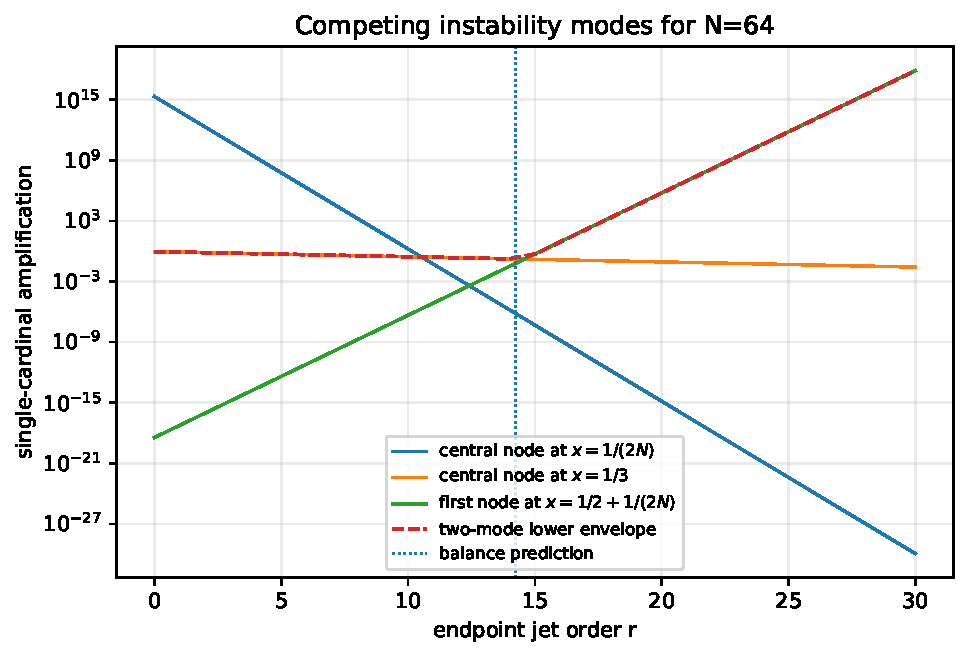
\includegraphics[width=0.82\textwidth]{figures/cardinal_modes_N64.pdf}
\caption{Three explicit value-cardinal modes for $N=64$.  Increasing $r$ suppresses the
half-cell and $x=1/3$ modes but amplifies the first-interior-node mode.  The dashed envelope
used in \cref{thm:all-r} never becomes small.}
\label{fig:cardinal-modes}
\end{figure}

\subsection{Fixing derivatives at every node can be worse}

A different reading of ``fixing higher derivatives'' is global confluent Hermite
interpolation: prescribe values and derivatives at every grid node.  Even the first-order
case squares the dominant Lagrange cardinal.

Let $\mathcal H_Nf$ be the degree-$2N+1$ polynomial matching $f$ and $f'$ at all
$x_j=j/N$.  If $\ell_j$ is the ordinary full-grid cardinal, the cardinal multiplying a
perturbation of the value $f_j$ is
\begin{equation}
 h_j(x)=\bigl[1-2\ell_j'(x_j)(x-x_j)\bigr]\ell_j(x)^2.
 \label{eq:Hermite-value-cardinal}
\end{equation}

\begin{theorem}[First-order global Hermite amplification]
\label{thm:global-hermite}
Let $N$ be even and $j=N/2$.  At $x=1/(2N)$ one has
$\ell_j'(x_j)=0$ and
\begin{equation}
 |\ell_j(1/(2N))|
 =\frac{\Gamma(N+\tfrac12)}
 {2\sqrt\pi(\tfrac N2-\tfrac12)\Gamma(N/2+1)^2}
 \sim \frac{\sqrt2}{\pi}\frac{2^N}{N^2}.
 \label{eq:full-central-cardinal}
\end{equation}
Consequently the value-data part of the first-order global Hermite Lebesgue constant obeys
\begin{equation}
 \Lambda_N^{C^1\text{-Hermite}}
 \ge |h_{N/2}(1/(2N))|
 \sim \frac{2}{\pi^2}\frac{4^N}{N^4}.
 \label{eq:Hermite-square-growth}
\end{equation}
This lower bound applies even when all derivative data are exact and held fixed.
\end{theorem}

\begin{proof}
The derivative $\ell_{N/2}'(x_{N/2})$ is the symmetric sum
$N\sum_{k\ne N/2}(N/2-k)^{-1}=0$.  The gamma product in
\eqref{eq:full-central-cardinal} follows by evaluating the full-node cardinal at
$Nx=1/2$.  Equation \eqref{eq:Hermite-value-cardinal} then reduces to $\ell_j^2$ at this
point, and Stirling's formula gives the asymptotic.
\end{proof}

The conclusion is not that derivative information is useless.  It is that forcing more
confluent conditions into one global equispaced polynomial inherits, and can magnify, the
same cardinal geometry.  Local Hermite interpolation behaves differently because its
cardinals never span an increasing number of cells.

\section{A two-mode balancing law for the favorable jet window}
\label{sec:balance}

The operator is unstable for every $r$, yet the exact Fabius and Rvachev data exhibit a
narrow range in which large cardinal terms cancel unusually well.  A useful prediction
comes from balancing two boundary mechanisms rather than minimizing the rigorous envelope
in \cref{thm:all-r}.

Use the fixed-$r$ half-cell mode from \eqref{eq:fixed-cardinal-asymptotic}, whose leading
logarithm is
\begin{equation}
 N\log2+r(\log2-\log N),
 \label{eq:half-leading-log}
\end{equation}
and the near-central first-node mode \eqref{eq:B-asympt}, whose leading logarithm is
\begin{equation}
 -N\log2+r(\log N-\log4).
 \label{eq:near-leading-log}
\end{equation}
Equating \eqref{eq:half-leading-log} and \eqref{eq:near-leading-log} gives
\begin{equation}
 \boxed{
 r_{\mathrm{bal}}(N)=
 \frac{2N\log2}{2\log N-3\log2}.}
 \label{eq:r-balance}
\end{equation}
For $N=2^n$ this simplifies exactly to
\begin{equation}
 r_{\mathrm{bal}}(2^n)=\frac{2^{n+1}}{2n-3}
 \sim \frac{N\log2}{\log N}.
 \label{eq:r-balance-dyadic}
\end{equation}

\begin{figure}[htbp]
\centering
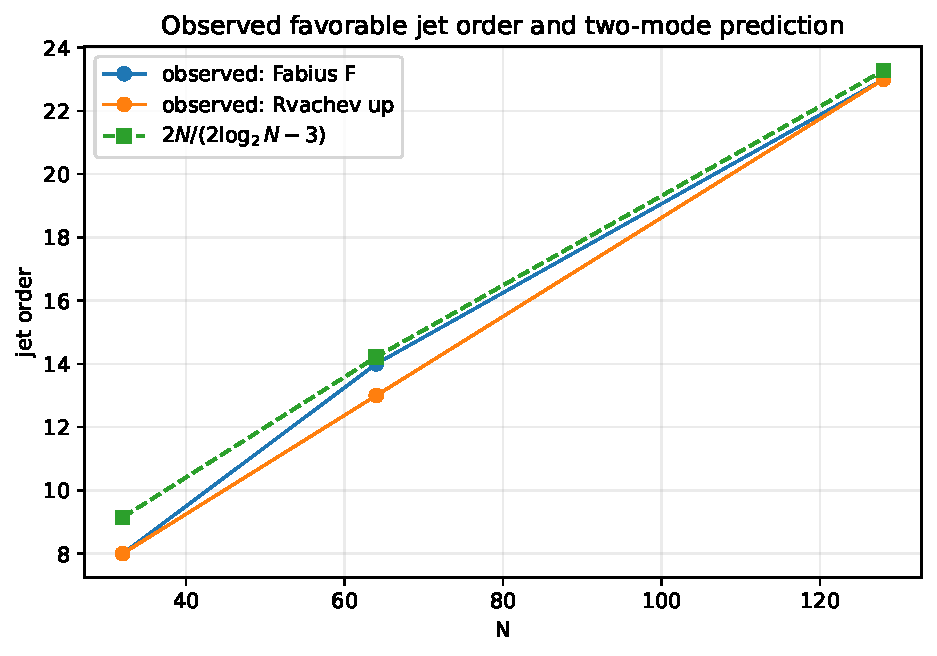
\includegraphics[width=0.78\textwidth]{figures/balancing_law.pdf}
\caption{Observed minimizing orders in the scanned windows versus
$r_{\rm bal}(N)=2N/(2\log_2N-3)$.  The agreement is much closer than a generic dimensional
argument would suggest.}
\label{fig:balance}
\end{figure}

\begin{center}
\small
\begin{tabular}{@{}ccccc@{}}
\toprule
Target & $N$ & observed $r$ & $r_{\rm bal}$ & sampled best error\\
\midrule
$F$ & 32 & 8  & 9.143  & $7.62\times10^{-7}$\\
$\Up$ & 32 & 8 & 9.143 & $4.08\times10^{-5}$\\
$F$ & 64 & 14 & 14.222 & $1.78\times10^{-6}$\\
$\Up$ & 64 & 13 & 14.222 & $2.12\times10^{-4}$\\
$F$ & 128 & 23 & 23.273 & $3.98\times10^{-3}$\\
$\Up$ & 128 & 23 & 23.273 & $5.31$\\
\bottomrule
\end{tabular}
\end{center}

\begin{warning}
The balance law predicts a favorable order for the particular data, not a small Lebesgue
constant.  At $r\asymp N/\log N$, the $x=1/3$ cardinal from \eqref{eq:mode-A} is still
exponentially large.  The observed accuracy therefore relies on highly structured
cancellation among exact Fabius values.  Such cancellation is sensitive to perturbations.
\end{warning}

\section{Remainders, derivative growth, and dyadic hierarchy}
\label{sec:remainder}

\subsection{The classical Hermite remainder is formally exact but practically weak}

\begin{proposition}[Endpoint-flat remainder]
\label{prop:remainder}
If $f\in C^{N+2r+1}[0,1]$, then for each $x\in[0,1]$ there is $\xi_x\in(0,1)$ such that
\begin{equation}
 f(x)-H_{N,r}f(x)
 =\frac{f^{(N+2r+1)}(\xi_x)}{(N+2r+1)!}
 x^{r+1}(x-1)^{r+1}
 \prod_{j=1}^{N-1}\left(x-\frac jN\right).
 \label{eq:Hermite-remainder}
\end{equation}
\end{proposition}

\begin{proof}
This is the standard confluent interpolation remainder for endpoint multiplicities $r+1$
and simple interior nodes.  The nodal polynomial has total degree
$2(r+1)+(N-1)=N+2r+1$.
\end{proof}

For $F$ or $\Up$, inserting \eqref{eq:derivative-norm} gives a factor
$2^{(N+2r+1)(N+2r+2)/2}/(N+2r+1)!$.  It is astronomically large and does not explain the
small-error windows.  This is not a contradiction: the derivative remainder uses one
extreme global derivative norm and ignores cancellation.  The failure is another analytic
signature of nowhere analyticity.

A better theoretical route would combine the explicit cardinal functions with the exact
Thue--Morse structure of the data, or use a Peano-kernel representation adapted to the
self-similar probability law.

\subsection{Nested dyadic correction identities}

Dyadic grids are nested, so successive interpolants have exact factorizations.

\begin{proposition}[Ordinary dyadic correction]
\label{prop:nested-ordinary}
Let $P_N$ and $P_{2N}$ be ordinary interpolants to the same function on the two nested
combs.  Then
\begin{equation}
 P_{2N}(x)-P_N(x)
 =\omega_N(x)R_{N-1}(x),
 \qquad
 \omega_N(x)=\prod_{j=0}^{N}\left(x-\frac jN\right),
 \label{eq:nested-ordinary}
\end{equation}
where $R_{N-1}\in\Pi_{N-1}$ is determined by the $N$ midpoint surpluses
$f((2j+1)/(2N))-P_N((2j+1)/(2N))$.
\end{proposition}

\begin{proposition}[Endpoint-flat dyadic correction]
\label{prop:nested-flat}
For fixed $r$,
\begin{equation}
 H_{2N,r}(x)-H_{N,r}(x)
 =[x(1-x)]^{r+1}
 \prod_{j=1}^{N-1}\left(x-\frac jN\right)R_{N-1,r}(x),
 \label{eq:nested-flat}
\end{equation}
with $R_{N-1,r}\in\Pi_{N-1}$ determined by the new midpoint data.
\end{proposition}

\begin{proof}
Both differences vanish at every coarse node.  In the endpoint-flat case they also have
zeros of multiplicity $r+1$ at $0$ and $1$.  Degree counting leaves a quotient of degree at
most $N-1$, and the $N$ midpoint values determine it uniquely.
\end{proof}

The factors in \eqref{eq:nested-ordinary}--\eqref{eq:nested-flat} define a natural
hierarchical Runge diagnostic.  If the normalized midpoint quotient becomes large near the
boundary, the next global level is already signaling instability.  Because the Fabius
midpoint values are exact Thue--Morse rationals, this hierarchy can be studied without
roundoff and may admit arithmetic recurrences.

\section{High-precision numerical experiments}
\label{sec:numerics}

\subsection{Method and reproducibility}

The numerical pipeline has four safeguards.

\begin{enumerate}
\item Every interpolation datum is first computed as an exact rational by
\cref{alg:stream}.  The $\Up$ data are obtained by the exact fold \eqref{eq:up-fold}.
\item The endpoint-flat polynomial is evaluated by the interior barycentric formula
\eqref{eq:bary-Q}.  Working precision grows with $N$ and $r$; the largest scans used several
hundred decimal digits.
\item Errors are compared with exact rational values on a finer dyadic grid.  Tables labeled
level $K$ use $2^K+1$ check points.  They are sampled maximum errors, not certified continuous
suprema.
\item Symmetry, interpolation, endpoint jets, and exact low-level values are checked
independently.  Increasing the check-grid level changes the quoted maxima only in the last
reported digits for the displayed cases.
\end{enumerate}

The archive contains
\path{fabius_dyadic_interpolation_experiments.py}, all CSV data, and both PDF and PNG forms
of the figures.  The default mode is a manageable smoke test; \texttt{--mode report}
performs the expensive high-precision scans.

\subsection{Ordinary Runge growth and transient suppression}

\begin{center}
\small
\setlength{\tabcolsep}{4.5pt}
\begin{tabular}{@{}ccrrrrr@{}}
\toprule
Target & $N$ & $r=0$ & $r=1$ & $r=2$ & $r=4$ & $r=8$\\
\midrule
$F$ & 8  & $9.49\!\times\!10^{-3}$ & $1.75\!\times\!10^{-3}$ & $1.50\!\times\!10^{-3}$ & $1.64\!\times\!10^{-3}$ & $2.78\!\times\!10^{-2}$\\
$F$ & 16 & $3.80\!\times\!10^{-3}$ & $2.68\!\times\!10^{-4}$ & $1.37\!\times\!10^{-4}$ & $4.93\!\times\!10^{-5}$ & $1.44\!\times\!10^{-4}$\\
$F$ & 32 & $4.99$ & $1.82\!\times\!10^{-1}$ & $9.75\!\times\!10^{-3}$ & $1.11\!\times\!10^{-4}$ & $7.62\!\times\!10^{-7}$\\
$F$ & 64 & $3.59\!\times\!10^{7}$ & $6.26\!\times\!10^{5}$ & $1.68\!\times\!10^{4}$ & $3.18\!\times\!10^{1}$ & $4.76\!\times\!10^{-3}$\\
\midrule
$\Up$ & 8  & $2.02\!\times\!10^{-1}$ & $3.07\!\times\!10^{-2}$ & $1.96\!\times\!10^{-2}$ & $1.34\!\times\!10^{-2}$ & $2.55\!\times\!10^{-1}$\\
$\Up$ & 16 & $1.97\!\times\!10^{-1}$ & $2.67\!\times\!10^{-2}$ & $4.17\!\times\!10^{-3}$ & $9.85\!\times\!10^{-4}$ & $1.06\!\times\!10^{-2}$\\
$\Up$ & 32 & $4.50\!\times\!10^{2}$ & $1.46\!\times\!10^{1}$ & $6.76\!\times\!10^{-1}$ & $4.45\!\times\!10^{-3}$ & $4.08\!\times\!10^{-5}$\\
$\Up$ & 64 & $1.05\!\times\!10^{10}$ & $1.75\!\times\!10^{8}$ & $4.52\!\times\!10^{6}$ & $7.72\!\times\!10^{3}$ & $9.49\!\times\!10^{-1}$\\
\bottomrule
\end{tabular}
\captionof{table}{Sampled maximum errors on a level-$11$ dyadic check grid.  Here $r=0$ is
ordinary Lagrange interpolation.}
\label{tab:fixed-errors}
\end{center}

Ordinary interpolation looks innocuous at $N=8$ and $16$ but undergoes a dramatic transition
between $N=16$ and $N=32$.  The oscillation is concentrated in endpoint layers, as in the
classical Runge phenomenon.  Because the samples and comparison values are exact rationals,
this is a property of the global interpolant, not sample noise.

\begin{figure}[htbp]
\centering
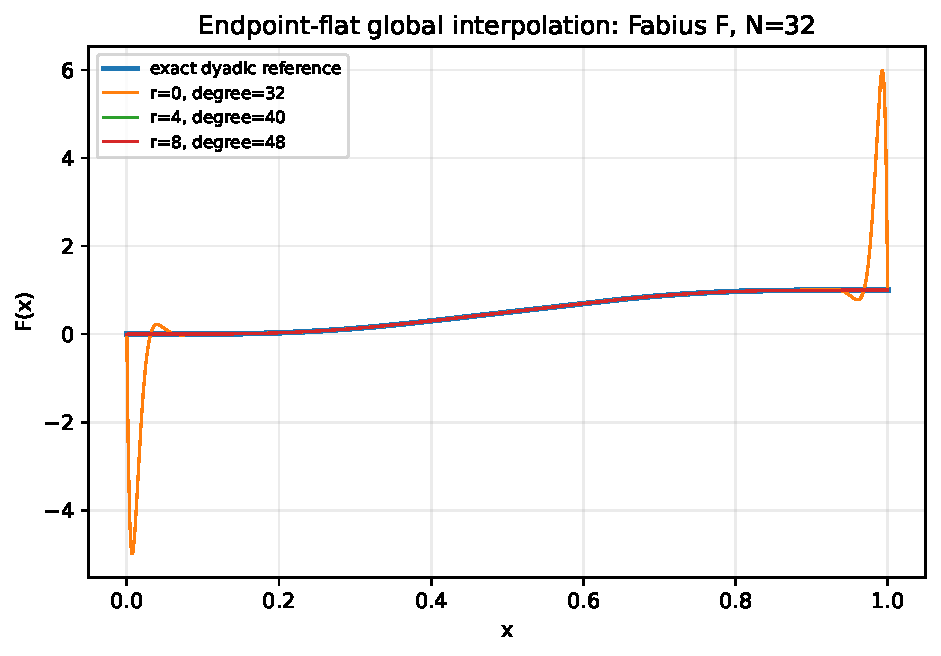
\includegraphics[width=0.82\textwidth]{figures/fabius_N32_interpolants.pdf}
\caption{Fabius interpolation on the $N=32$ comb.  Ordinary interpolation has already
entered a large boundary-layer regime.  Moderate endpoint constraints recover excellent
accuracy, but this improvement is temporary.}
\label{fig:F-N32}
\end{figure}

\begin{figure}[htbp]
\centering
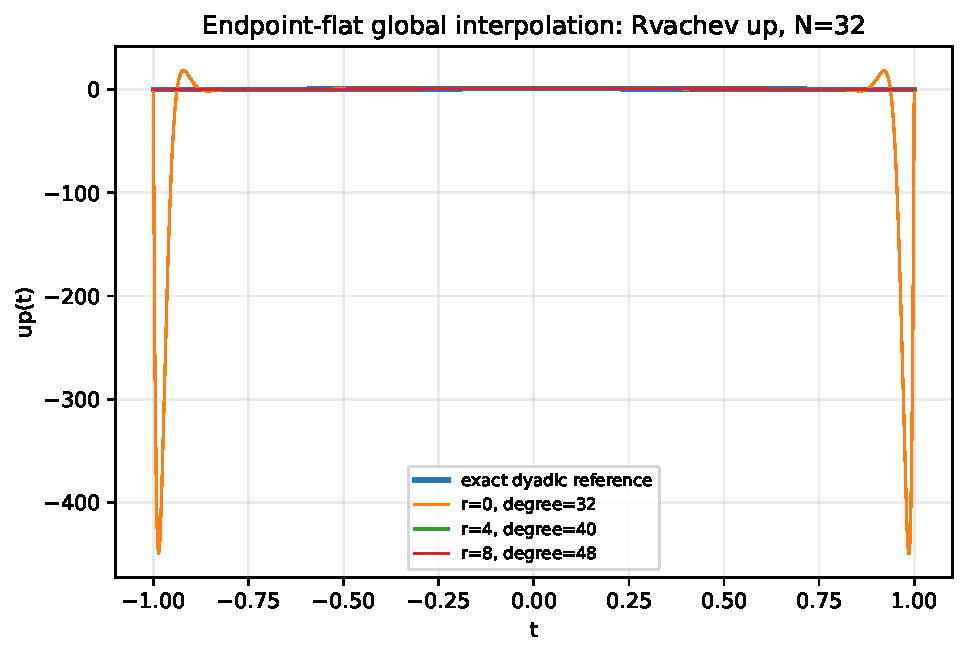
\includegraphics[width=0.82\textwidth]{figures/up_N32_interpolants.pdf}
\caption{The affine $N=32$ Rvachev experiment.  Evenness is exact, so the two endpoint
boundary layers are mirror images.}
\label{fig:up-N32}
\end{figure}

\subsection{The U-shaped jet scan}

At $N=64$, scanning all $0\le r\le20$ reveals the predicted tradeoff.

\begin{center}
\small
\begin{tabular}{@{}crr@{}}
\toprule
$r$ & sampled error for $F$ & sampled error for $\Up$\\
\midrule
0  & $3.59\times10^7$ & $1.05\times10^{10}$\\
4  & $3.18\times10^1$ & $7.72\times10^3$\\
8  & $4.76\times10^{-3}$ & $9.49\times10^{-1}$\\
10 & $1.55\times10^{-4}$ & $2.73\times10^{-2}$\\
12 & $8.30\times10^{-6}$ & $1.26\times10^{-3}$\\
13 & $1.94\times10^{-6}$ & $2.12\times10^{-4}$\\
14 & $1.78\times10^{-6}$ & $6.19\times10^{-4}$\\
16 & $7.79\times10^{-5}$ & $1.95\times10^{-2}$\\
18 & $3.25\times10^{-3}$ & $7.31\times10^{-1}$\\
20 & $1.72\times10^{-1}$ & $3.65\times10^{1}$\\
\bottomrule
\end{tabular}
\captionof{table}{Selected rows of the $N=64$ jet scan.}
\label{tab:jet64}
\end{center}

\begin{figure}[htbp]
\centering
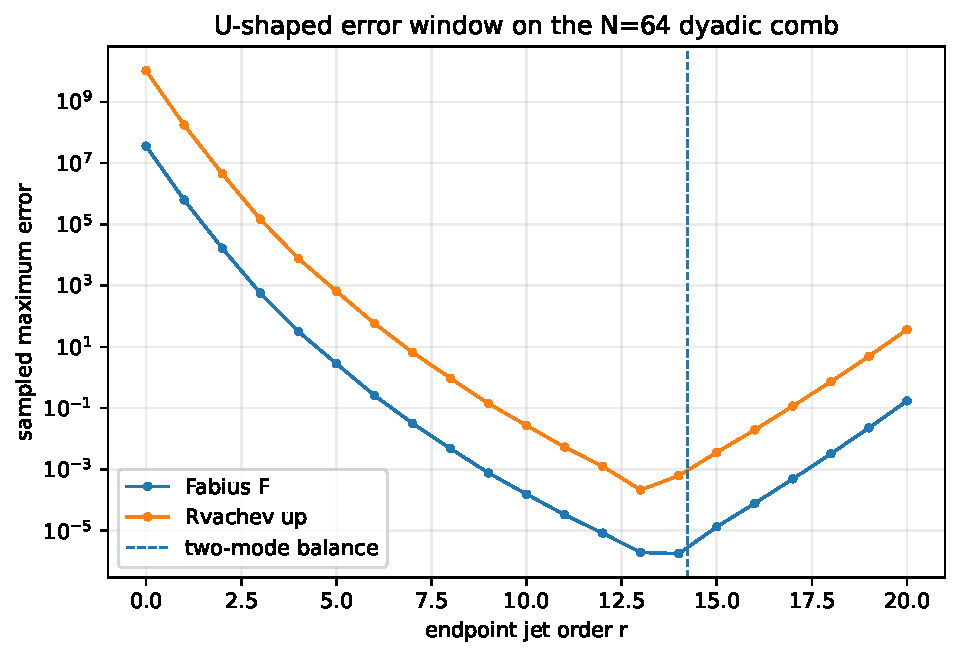
\includegraphics[width=0.80\textwidth]{figures/jet_order_scan_N64.pdf}
\caption{The error as a function of endpoint jet order is sharply U-shaped.  The vertical
line is $r_{\rm bal}(64)=128/9=14.22\ldots$.}
\label{fig:jet64}
\end{figure}

The same phenomenon at $N=128$ is less reassuring.  The favorable order remains almost
exactly the balancing prediction, but the minimum errors increase to about
$3.98\times10^{-3}$ for $F$ and $5.31$ for $\Up$.  Thus optimizing $r$ does not produce a
monotone convergent method in the tested range.

\subsection{Interpretation}

The data support four conclusions.

\begin{enumerate}
\item \emph{Runge phenomenon occurs for the specific functions.}  The ordinary global
interpolants develop rapidly growing endpoint oscillations.
\item \emph{Correct endpoint derivatives matter at finite degree.}  They remove the first
spurious jets and can improve errors by many orders of magnitude.
\item \emph{The benefit has a finite window.}  Once $r$ is too large, division by the tiny
endpoint factors in \eqref{eq:qj-F} amplifies near-boundary data.
\item \emph{Function-specific cancellation is not stability.}  The small errors near the
minimum coexist with exponentially large cardinal functions.  Perturbing exact samples by
even tiny relative errors can destroy the cancellation.
\end{enumerate}

\section{A stable cure on the same dyadic comb: local Hermite interpolation}
\label{sec:local}

The global polynomial is the source of the long-range cardinal coupling.  Keep the same
dyadic nodes but interpolate separately on each cell $[j/N,(j+1)/N]$.

For a fixed $s\ge0$, let $\mathcal H^{\rm loc}_{N,s}f$ be the piecewise polynomial of degree
$2s+1$ that matches $f^{(k)}$ at both ends of every cell for $0\le k\le s$.

\begin{theorem}[Local endpoint-Hermite error]
\label{thm:local-error}
For $f\in C^{2s+2}[0,1]$,
\begin{equation}
 \|f-\mathcal H^{\rm loc}_{N,s}f\|_\infty
 \le \frac{\|f^{(2s+2)}\|_\infty}{(2s+2)!}
 \left(\frac{1}{4N^2}\right)^{s+1}.
 \label{eq:local-general}
\end{equation}
Consequently,
\begin{equation}
 \boxed{
 \|F-\mathcal H^{\rm loc}_{N,s}F\|_\infty
 \le
 \frac{2^{(s+1)(2s+1)}}{(2s+2)!}\,N^{-2s-2}.}
 \label{eq:local-F-bound}
\end{equation}
For $N$ equal cells on $[-1,1]$,
\begin{equation}
 \boxed{
 \|\Up-\mathcal H^{\rm loc}_{N,s}\Up\|_\infty
 \le
 \frac{2^{\binom{2s+3}{2}}}{(2s+2)!}\,N^{-2s-2}.}
 \label{eq:local-up-bound}
\end{equation}
The local value and derivative cardinal functions have norms bounded independently of $N$.
\end{theorem}

\begin{proof}
On a cell $[a,b]$ of length $h$, the two-point Hermite remainder is
\[
 \frac{f^{(2s+2)}(\xi)}{(2s+2)!}(x-a)^{s+1}(x-b)^{s+1}.
\]
The absolute product is at most $(h^2/4)^{s+1}$.  For $F$, use $h=1/N$ and
\eqref{eq:derivative-norm}; the factor $4^{-(s+1)}$ reduces the derivative exponent to
$(s+1)(2s+1)$.  For $\Up$ on $[-1,1]$, $h=2/N$, so $h^2/4=N^{-2}$ and no further power of
four appears.  After rescaling a cell to $[0,1]$, the local cardinal basis depends only on
$s$, proving $N$-independent conditioning.
\end{proof}

For cubic Hermite interpolation ($s=1$), exact dyadic values and exact derivatives from
\eqref{eq:Fprime-up} give the following sampled errors.

\begin{center}
\small
\begin{tabular}{@{}rrrrrr@{}}
\toprule
$N$ & 4 & 8 & 16 & 32 & 64\\
\midrule
sampled error & $9.67\times10^{-4}$ & $5.03\times10^{-4}$ & $2.06\times10^{-5}$ & $2.29\times10^{-6}$ & $1.58\times10^{-7}$\\
\bottomrule
\end{tabular}
\captionof{table}{Piecewise cubic Fabius errors on a level-$12$ check grid.}
\label{tab:local-errors}
\end{center}

\begin{figure}[htbp]
\centering
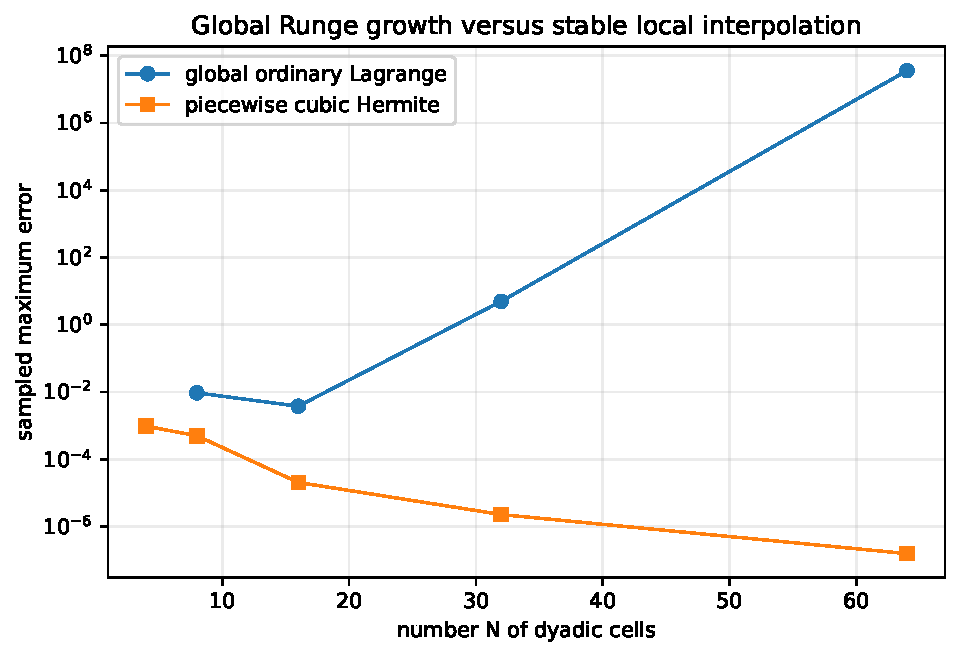
\includegraphics[width=0.80\textwidth]{figures/global_vs_local.pdf}
\caption{Ordinary global interpolation becomes catastrophic, while the cellwise cubic
method converges steadily on the same dyadic samples.}
\label{fig:global-local}
\end{figure}

Other stable choices that retain equispaced data include low-degree splines, Floater--Hormann
rational interpolation, constrained least squares, and oversampled polynomial frames.  If a
single global polynomial is essential, oversampling and regularization are more promising
than adding exact confluent conditions at every sample.

\section{Connections with the surrounding Fabius--Rvachev theory}
\label{sec:connections}

\subsection{Thue--Morse signs and exact interpolation coefficients}

Every coefficient of $P_N^F$ and $H^F_{N,r}$ is rational and can be expanded into finite
sums involving $\eps_h$.  Combining \eqref{eq:newton-forward} with
\eqref{eq:exact-dyadic-d} gives a triple finite sum for the Newton coefficients
$\Delta^kF(0)$.  Prouhet cancellation annihilates low-degree polynomial parts of complete
Thue--Morse blocks.  This suggests that the unexpectedly small function-specific error near
$r_{\rm bal}$ is not accidental: large cardinals may cancel against blockwise signed moment
identities in the exact data.

A tractable first target is the midpoint surplus
\begin{equation}
 \sigma_{N,j}=F\!\left(\frac{2j+1}{2N}\right)
 -P_N^F\!\left(\frac{2j+1}{2N}\right),
 \label{eq:midpoint-surplus}
\end{equation}
which is rational and determines the entire correction in
\eqref{eq:nested-ordinary}.  Its numerator should admit a block decomposition governed by
the Thue--Morse polynomial
$\prod_{k=0}^{n-1}(1-z^{2^k})$.

\subsection{Additive versus geometric Lagrange weights}

The repository's $q$-binomial interpolation uses geometric nodes and weights naturally
expressed through Gaussian binomial coefficients.  The additive interior comb instead has
the binomial barycentric weights \eqref{eq:interior-weights}.  Both are manifestations of a
Vandermonde inverse, but with different node groups:
\begin{center}
\begin{tabular}{@{}lll@{}}
\toprule
Geometry & Nodes & Natural weights\\
\midrule
additive dyadic comb & $j/2^n$ & $(-1)^{j-1}\binom{N-2}{j-1}$\\
geometric/$q$ comb & $q^j$ or $-2^j$ & Gaussian-binomial products\\
\bottomrule
\end{tabular}
\end{center}
A mixed transform could interpolate across additive location while filtering across dyadic
scale.  The nested surplus polynomial in \eqref{eq:nested-flat} is a natural place to search
for such an additive--multiplicative bridge.

\subsection{Fourier sinc products and local approximation}

The infinite sinc product for $\widehat{\Up}$ explains the extraordinary smoothness and
provides moment and derivative information.  For local interpolation it yields useful
Fourier-domain error estimates: the cellwise operator acts as a compactly supported
quasi-interpolant whose multiplier can be compared with the sinc product near the origin.
This may sharpen the elementary derivative bound \eqref{eq:local-up-bound}, especially when
$s$ grows slowly with $N$.

By contrast, a global polynomial has no compactly localized Fourier response.  Its
endpoint oscillations correspond to broad spectral leakage, another way to see why the
compact-support structure of $\Up$ is better respected by local atomic-function or spline
bases.

\subsection{Lambert--W endpoint phase}

The repository proves that the sharp small-$x$ asymptotic of $F(x)$ contains a nonconstant
periodic correction evaluated at a lower-Lambert phase.  Global interpolation errors are
largest in boundary layers whose locations shrink with $N$.  Substituting the empirical
maximizer $x_N$ into the lower-Lambert phase may reveal a log-periodic drift in both the
error and the integer offset
$r_{\rm opt}-r_{\rm bal}$.  This would connect a purely numerical-analysis phenomenon with
the endpoint saddle structure.

\subsection{Bell and Bernoulli polynomials}

The moments $c_k,d_k$ have Bernoulli recurrences, while saddle corrections are organized by
Bell-polynomial algebra in the repository.  Two possible uses in interpolation are:

\begin{enumerate}
\item express the exact endpoint jets \eqref{eq:jet-defect} as Bell-polynomial transforms of
the moment generating series;
\item derive asymptotic expansions of the gamma-cardinal modes beyond leading order, then
balance them to obtain corrections to \eqref{eq:r-balance}.
\end{enumerate}

The second program is especially concrete.  Stirling--Bernoulli expansions of
\eqref{eq:fixed-cardinal-exact} and \eqref{eq:mode-B} should produce
\begin{equation}
 r_{\rm opt}(N)=\frac{2N\log2}{2\log N-3\log2}
 +\frac{a_1N}{(\log N)^2}+a_0+\cdots,
 \label{eq:r-corrected-form}
\end{equation}
with coefficients modified by function-specific Thue--Morse cancellation.

\subsection{Inverse Fabius interpolation}

The inverse $F^{-1}$ has infinite endpoint slopes rather than flat endpoints.  Direct
polynomial interpolation of $F^{-1}$ on a uniform value comb should therefore have a
different but equally severe endpoint problem.  A more natural scheme is parametric:
interpolate the exact pairs $(F(j/N),j/N)$ or apply a variable transformation informed by
the lower-Lambert asymptotic.  The endpoint-flat analysis here supplies a warning: imposing
large derivative data globally is unlikely to be stable; local rational or monotone Hermite
methods are preferable.

\section{Conjectures}
\label{sec:conjectures}

The following statements are deliberately separated from the proved results.

\begin{conjecture}[Two-mode optimal-jet law]
\label{conj:optimal-jet}
Let $r_N^F$ and $r_N^{\Up}$ minimize the sampled or true uniform error among the endpoint-flat
global interpolants.  Along dyadic $N=2^n$,
\begin{equation}
 r_N^F=\frac{2N}{2n-3}+\bigO(1),
 \qquad
 r_N^{\Up}=\frac{2N}{2n-3}+\bigO(1).
 \label{eq:conj-optimal-r}
\end{equation}
A refined version has bounded oscillatory corrections determined by a Thue--Morse or
lower-Lambert phase.
\end{conjecture}

\begin{conjecture}[Failure of optimized global convergence]
\label{conj:optimized-failure}
Define
\[
 E_N^F=\inf_{r\ge0}\|F-H^F_{N,r}\|_\infty,
 \qquad
 E_N^{\Up}=\inf_{r\ge0}\|\Up-H^{\Up}_{N,r}\|_\infty.
\]
Then neither sequence tends to zero along all dyadic $N$.  More strongly,
\begin{equation}
 \limsup_{n\to\infty}E_{2^n}^F>0,
 \qquad
 \limsup_{n\to\infty}E_{2^n}^{\Up}=+\infty.
 \label{eq:conj-nonconvergence}
\end{equation}
The $N=128$ deterioration is the first numerical indication, not a proof.
\end{conjecture}

\begin{conjecture}[Dyadic surplus arithmetic]
\label{conj:surplus}
After multiplication by the natural common denominator from the dyadic moment formulas, the
midpoint surplus vector $\sigma_{N,j}$ in \eqref{eq:midpoint-surplus} factors into a finite
binomial transform of a Thue--Morse block.  Its sign changes and largest boundary entries
obey a recursion of depth $n$.
\end{conjecture}

\begin{conjecture}[Higher global confluent amplification]
\label{conj:higher-hermite}
For global Hermite interpolation matching derivatives through a fixed order $s\ge1$ at all
$N+1$ equidistant nodes, the value-data Lebesgue constant has a lower bound of the form
\begin{equation}
 \Lambda_{N,s}^{\rm confluent}
 \ge C_s\frac{2^{(s+1)N}}{N^{\alpha_s}}
 \label{eq:conj-higher-hermite}
\end{equation}
for explicit $\alpha_s$.  Theorem~\ref{thm:global-hermite} is the case $s=1$ with
$\alpha_1=4$.
\end{conjecture}

\begin{conjecture}[Lambert phase locking]
\label{conj:phase}
Let $x_N$ be the leftmost point at which the optimized interpolation error reaches its
maximum.  The lower-Lambert phase associated with $x_N$ has a limiting rotation modulo one,
and the fluctuations of
$r_N-r_{\rm bal}(N)$ and $\log E_N$ are continuous periodic functions of that phase.
\end{conjecture}

\section{Promising research directions}
\label{sec:future}

\subsection{Prove function-specific divergence}

The most important open step is to pass from operator instability to a lower bound for the
actual Fabius data.  Three routes look promising.

\begin{enumerate}
\item Insert the exact dyadic formula into a selected cardinal evaluation and exploit
Thue--Morse block cancellation until one dominant term remains.
\item Analyze the Newton coefficients $\Delta^kF(0)$ by a two-variable saddle method in
$k$ and $n$.
\item Use the nested surplus factorization and prove that a boundary surplus cannot remain
small at all dyadic levels.
\end{enumerate}

\subsection{Obtain a corrected balance expansion}

Use Stirling--Bernoulli series for the two cardinal modes and match not only the exponential
terms but the powers of $N$ and constants.  Compare the resulting correction with exact
high-precision minimizers for $N=256$ and $512$.  The formula
\eqref{eq:r-corrected-form} should be tested separately for $F$ and $\Up$.

\subsection{Design stable dyadic approximants}

The same exact samples can support methods with much better conditioning:

\begin{itemize}
\item piecewise Hermite interpolation of adaptive local order;
\item compactly supported Rvachev atomic-function quasi-interpolation;
\item monotone rational Hermite interpolation for $F$;
\item oversampled polynomial least squares with degree $m\ll N$;
\item polynomial frames or constrained minimax reconstruction;
\item rational barycentric methods with poles kept away from $[0,1]$.
\end{itemize}

A useful benchmark suite should report approximation error, Lebesgue/condition number,
monotonicity, symmetry defect, and exact-data sensitivity separately.

\subsection{Exploit the dyadic hierarchy}

The correction polynomials in \eqref{eq:nested-ordinary} and \eqref{eq:nested-flat} give an
adaptive algorithm: compute midpoint surpluses exactly, stop refining cells whose normalized
surplus is small, and switch from global to local interpolation when the boundary quotient
begins to grow.  This creates a mathematically transparent Runge detector specialized to
nested dyadic data.

\subsection{Formalize the new finite theorems}

The factorization theorem, cardinal formulas, gamma-product identities, and all-order case
split are finite algebra and real asymptotics well suited to Lean.  A suggested sequence is:

\begin{enumerate}
\item confluent interpolation uniqueness and divisibility by endpoint powers;
\item interior barycentric weights on an arithmetic progression;
\item exact gamma products for the three selected cardinals;
\item Stirling-ratio asymptotics;
\item the uniform-in-$r$ instability theorem;
\item local Hermite remainder and Fabius derivative specialization.
\end{enumerate}

This would extend the repository's current geometric Lagrange formalization to additive
comb interpolation without duplicating it.

\section{Summary}

Global equispaced interpolation of the Fabius and Rvachev functions is a particularly sharp
laboratory for Runge instability.  Exact arithmetic removes sample uncertainty; symmetry
reduces the polynomials to half-size forms; and endpoint flatness offers seemingly ideal
Hermite data.  Yet the geometry of the comb dominates.  A fixed number of endpoint
constraints changes exponential cardinal growth only by powers of $N$, while a growing
number transfers the instability from central data to near-endpoint data.  Matching
first derivatives at every node can square the exponential growth.

The surprising positive result is not stability but structure.  The exact smoothstep
factorization exposes the mechanism, and a two-mode calculation predicts the narrow
function-specific accuracy window almost perfectly.  That window should be treated as a
frontier cancellation phenomenon, probably tied to Thue--Morse arithmetic and endpoint
Lambert phases, rather than as a reliable numerical method.  On the same dyadic comb,
local Hermite interpolation gives the genuine cure: bounded local conditioning and explicit
algebraic convergence.

\appendix

\section{Gamma-product calculations}
\label{app:gamma}

\subsection{Interior central cardinal at a half cell}

For interior nodes $1,\ldots,N-1$ in the scaled variable $y=Nx$ and $j=N/2$,
\[
 \ell_j^\circ(y/N)=\prod_{\substack{1\le k\le N-1\\k\ne j}}
 \frac{y-k}{j-k}.
\]
At $y=1/2$,
\[
 \prod_{k=1}^{N-1}|k-1/2|=\frac{\Gamma(N-1/2)}{\Gamma(1/2)},
\]
and deleting the $j$ factor divides by $j-1/2$.  The denominator is
$(j-1)!(N-1-j)!=\Gamma(N/2)^2$, yielding
\eqref{eq:fixed-cardinal-exact}.

\subsection{The one-third mode}

At $y=N/3$,
\[
 \prod_{k=1}^{N-1}(N/3-k)
 =\frac{\Gamma(N/3)}{\Gamma(1-2N/3)}.
\]
Reflection gives
\[
 \frac{1}{|\Gamma(1-2N/3)|}
 =\frac{\Gamma(2N/3)|\sin(2\pi N/3)|}{\pi}
 =\frac{\sqrt3}{2\pi}\Gamma(2N/3),
\]
because dyadic $N$ is not divisible by $3$.  Removing the central factor
$|N/3-N/2|=N/6$ and dividing by $\Gamma(N/2)^2$ gives \eqref{eq:mode-A}.
The exponential part of the gamma ratio is
\[
 \exp\!\left\{N\left[
 \frac13\log\frac13+\frac23\log\frac23-\log\frac12
 \right]\right\}
 =\e^{N(\log2-H(1/3))}.
\]

\subsection{The near-central boundary-node mode}

For $j=1$ and $y=(N+1)/2$,
\[
 \left|\prod_{k=2}^{N-1}(y-k)\right|
 =\left[\frac{\Gamma(N/2-1/2)}{\Gamma(1/2)}\right]^2.
\]
The denominator is $(N-2)!=\Gamma(N-1)$.  Also
\[
 \frac{x(1-x)}{x_1(1-x_1)}
 =\frac{(1/4)(1-N^{-2})}{N^{-1}(1-N^{-1})}
 =\frac{N+1}{4},
\]
proving \eqref{eq:mode-B}.  The duplication formula gives
\[
 \frac{\Gamma(N/2-1/2)^2}{\pi\Gamma(N-1)}
 =\frac{2^{2-N}}{\sqrt\pi}
 \frac{\Gamma((N-1)/2)}{\Gamma(N/2)}
 \sim2^{2-N}\sqrt{\frac{2}{\pi N}}.
\]

\section{Core exact-arithmetic pseudocode}
\label{app:algorithm}

\begin{lstlisting}[style=pythonstyle,caption={Streaming the exact dyadic Fabius comb.}]
def fabius_grid_exact(level):
    n = level
    N = 2**n
    d = exact_half_moments(n)       # Fractions
    S = [0] * (n + 1)              # integer Thue--Morse prefix moments
    scale = Fraction(1, 2**(n*(n-1)//2) * factorial(n))
    values = []

    for a in range(N + 1):
        total = sum(comb(n, j) * d[j] * S[n-j]
                    for j in range(n + 1))
        values.append(scale * total)
        if a == N:
            break

        eps = (-1)**popcount(a)
        next_S = [0] * (n + 1)
        next_S[0] = S[0] + eps
        for k in range(1, n + 1):
            next_S[k] = sum(comb(k, q) * S[q]
                            for q in range(k + 1))
        S = next_S
    return values
\end{lstlisting}

The actual program adds caching, reflection checks, exact derivative data, high-precision
barycentric interpolation, CSV output, figures, cardinal-mode formulas, and command-line
options.

\section{Reproduction manifest}
\label{app:manifest}

The ZIP archive contains:

\begin{longtable}{@{}p{0.43\textwidth}p{0.50\textwidth}@{}}
\toprule
Path & Purpose\\
\midrule
\endfirsthead
\toprule
Path & Purpose\\
\midrule
\endhead
\path{fabius_dyadic_interpolation_report.tex} & Complete LaTeX source.\\
\path{fabius_dyadic_interpolation_report.pdf} & Rendered report.\\
\path{fabius_dyadic_interpolation_experiments.py} & Exact rational and high-precision numerical experiments, with extensive comments.\\
\path{data/fixed_order_errors.csv} & Errors for $r\in\{0,1,2,4,8\}$ and $N\le64$.\\
\path{data/jet_scan_N64.csv} & Complete $0\le r\le20$ scan for both targets.\\
\path{data/jet_scan_N128_window.csv} & Focused high-precision scan around the predicted favorable order.\\
\path{data/observed_optimal_orders.csv} & Comparison with the balancing law.\\
\path{data/piecewise_cubic_errors.csv} & Stable local-Hermite comparison.\\
\path{data/cardinal_modes.csv} & Explicit theoretical cardinal values near $r_{\rm bal}$.\\
\path{figures/*.pdf}, \path{figures/*.png} & Vector figures used in the report and raster copies for inspection.\\
\path{README.md} & Build and execution instructions.\\
\bottomrule
\end{longtable}

To rebuild the numerical outputs:
\begin{lstlisting}[style=pythonstyle]
python fabius_dyadic_interpolation_experiments.py \
    --mode report --check-level 11 --output-dir reproduced
\end{lstlisting}
The full scan is intentionally expensive because it uses exact input arithmetic and hundreds
of decimal digits for the most ill-conditioned cases.  The default \texttt{quick} mode
provides a smaller verification run.

\section{Corpus coverage matrix}
\label{app:corpus}

\begin{longtable}{@{}p{0.25\textwidth}p{0.32\textwidth}p{0.35\textwidth}@{}}
\toprule
Corpus component & Relevant existing content & Nonduplication conclusion\\
\midrule
\endfirsthead
\toprule
Corpus component & Relevant existing content & Nonduplication conclusion\\
\midrule
\endhead
Current primary exposition & Exact dyadic values; derivatives and flatness; moments; Fourier--Legendre least squares; geometric Lagrange and Richardson; lower-Lambert endpoint asymptotics. & No additive-comb Runge or endpoint-flat Hermite analysis.\\
Current frontier volume & Non-formalized asymptotics, $q$-filters, dyadic formulas, approximation ideas, and conjectures. & No theorem equivalent to \cref{thm:factorization,thm:all-r,thm:global-hermite}.\\
Historical primary and supplements & Earlier versions of function theory, exact arithmetic, and asymptotics. & Keyword and passage audit found no ordinary/Hermite dyadic-comb study.\\
Historical dyadic and $q$ studies & Alternative exact formulas, Gaussian coefficients, convergence accelerators. & Node geometry and objectives differ from additive global interpolation.\\
Historical frontier consolidation & Legendre expansion and best polynomial approximation among many frontier topics. & Orthogonal approximation is distinct from interpolation and Runge conditioning.\\
Paper-source directories & Arias de Reyna, lacunary products, Fabius and arithmetic source papers. & Supply background identities; no matching endpoint-jet Runge result found.\\
\bottomrule
\end{longtable}

\begin{thebibliography}{99}

\bibitem{proveitprimary}
V.~Reshetnikov,
\newblock \emph{The Fabius Function and Rvachev's Up-Function: Exact arithmetic,
probability, Fourier analysis, and corrected sharp asymptotics},
\newblock current human-readable synthesis in the \texttt{ProveIt} repository,
\path{Analysis/FabiusFunction/docs/Fabius_Function_and_Rvachev_Up/}, snapshot 28 August 2026.

\bibitem{proveitfrontier}
V.~Reshetnikov,
\newblock \emph{Non-Formalized Research Frontiers for the Fabius Function},
\newblock \texttt{ProveIt} repository,
\path{Analysis/FabiusFunction/docs/non-formalized-research-frontiers/}, snapshot 28 August 2026.

\bibitem{jessen1935}
B.~Jessen and A.~Wintner,
\newblock Distribution functions and the Riemann zeta function,
\newblock \emph{Transactions of the American Mathematical Society} \textbf{38} (1935), 48--88.

\bibitem{fabius1966}
J.~Fabius,
\newblock A probabilistic example of a nowhere analytic $C^\infty$-function,
\newblock \emph{Zeitschrift fuer Wahrscheinlichkeitstheorie und Verwandte Gebiete}
\textbf{5} (1966), 173--174.
\newblock DOI: \nolinkurl{10.1007/BF00536652}.

\bibitem{rvachev1990}
V.~A.~Rvachev,
\newblock Compactly supported solutions of functional-differential equations and their applications,
\newblock \emph{Russian Mathematical Surveys} \textbf{45} (1990), no.~1, 87--120.

\bibitem{arias1982}
J.~Arias de Reyna,
\newblock Definicion y estudio de una funcion indefinidamente diferenciable de soporte compacto,
\newblock \emph{Revista de la Real Academia de Ciencias Exactas, Fisicas y Naturales de Madrid}
\textbf{76} (1982), no.~1, 21--38;
English translation, arXiv:\nolinkurl{1702.05442} (2017).

\bibitem{arias2018}
J.~Arias de Reyna,
\newblock Arithmetic of the Fabius function,
\newblock \emph{INTEGERS} \textbf{18} (2018), Article A51;
arXiv:\nolinkurl{1702.06487}, version 3.

\bibitem{haugland2016}
J.~K.~Haugland,
\newblock Evaluating the Fabius function,
\newblock arXiv:\nolinkurl{1609.07999} (2016).

\bibitem{runge1901}
C.~Runge,
\newblock Ueber empirische Funktionen und die Interpolation zwischen aequidistanten Ordinaten,
\newblock \emph{Zeitschrift fuer Mathematik und Physik} \textbf{46} (1901), 224--243.

\bibitem{mills1992}
T.~M.~Mills and S.~J.~Smith,
\newblock The Lebesgue constant for Lagrange interpolation on equidistant nodes,
\newblock \emph{Numerische Mathematik} \textbf{61} (1992), 111--115.
\newblock DOI: \nolinkurl{10.1007/BF01385500}.

\bibitem{berrut2004}
J.-P.~Berrut and L.~N.~Trefethen,
\newblock Barycentric Lagrange interpolation,
\newblock \emph{SIAM Review} \textbf{46} (2004), no.~3, 501--517.
\newblock DOI: \nolinkurl{10.1137/S0036144502417715}.

\bibitem{platte2011}
R.~B.~Platte, L.~N.~Trefethen, and A.~B.~J.~Kuijlaars,
\newblock Impossibility of fast stable approximation of analytic functions from equispaced samples,
\newblock \emph{SIAM Review} \textbf{53} (2011), no.~2, 308--318.
\newblock DOI: \nolinkurl{10.1137/090774707}.

\bibitem{adcock2023}
B.~Adcock and A.~Shadrin,
\newblock Fast and stable approximation of analytic functions from equispaced samples via polynomial frames,
\newblock \emph{Constructive Approximation} \textbf{57} (2023), 257--294.
\newblock DOI: \nolinkurl{10.1007/s00365-022-09593-2}.

\end{thebibliography}

\end{document}
